\scanpage{56}
% archive foliation: 55
U N I V E R S I T E

DES SCIENCES ET TECHNIQUES

DU LANGUEDOC

\texttt{------------}

MONTPELLIER, le 15 Juin 1978

Service de la Scolarité

MR/GJ

Diffusion : Liste H

N° 3758

\uline{AVIS DE SOUTENANCE D'UNE THESE DE DOCTORAT D'ETAT}

\uline{Nom et prénom du candidat} : WALTER Philippe

\uline{Titre de la thèse} : Recherches écologiques et biologiques sur les Scarabéides Co-\\
prophages d'une savane du Zaïre.

\uline{Date, heure et lieu de soutenance prévus} : 3 JUILLET 1978 à 9 Heures 30 mn

Salle de cours n° 6, U.S.T.L.

\uline{Nom du Directeur de thèse} : Monsieur le Professeur Renaud PAULIAN.

\uline{Désignation du laboratoire où la thèse est préparée} : Zoologie (Professeur LEGENDRE)

\uline{Résumé de la thèse} : Les recherches ont été effectuées sur le Plateau Bateke zaïrois.
Les résultats sont présentés en trois parties :

1) le peuplement (composition d'ensemble, aspects biogéographiques, répartition dans
les différentes formations végétales, fluctuations des densités de population,
sex-ratio)

2) observations autoécologiques et biologiques (préférences trophiques, heures
d'activité, éthologie)

3) morphologie larvaire : description détaillée de 12 larves.

\uline{Durée approximative des recherches ayant abouti à la thèse} : 5 ans 1/2.

\uline{Noms des Rapporteurs} :

\diagram{\begin{tabular}{ll}
PAULIAN R. & , Professeur, Zoogéographie, Rectorat BORDEAUX\\
LAMOTTE M. & , Professeur, Ecologie, Ecole Normale Supérieure PARIS\\
LEGENDRE R. & , Professeur, Zoologie Ecologie, U.S.T.L.
\end{tabular}}

\uline{Composition du jury} :

\diagram{\begin{tabular}{ll}
LEGENDRE R. & , Professeur, Zoologie Ecologie, U.S.T.L.\\
& (Président)\\[1ex]
PAULIAN R. & , Professeur, Zoogéographie, Rectorat BORDEAUX\\
LAMOTTE M. & , Professeur, Ecologie, Ecole Normale Supérieure PARIS\\
& (Membres extérieurs choisis en raison de leur compétence scientifique)\\[1ex]
EUZET L. & , Professeur, Parasitologie, U.S.T.L.\\
& (Membre étranger à la spécialité du candidat)\\
LUMARET J.-P. & , Maître-assistant, Biogéographie, Univ. MONTPELLIER III.\\
BARAUD J. & ., Professeur, Biochimie, Univ. BORDEAUX
\end{tabular}}

Le Secrétaire Général,

\figure{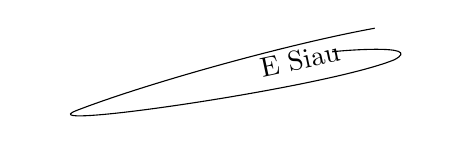
\begin{tikzpicture}
\node[rotate=12] at (1.55,.25){\unsure{E Siau}};
\draw (2.5,.65) .. controls (1.4,.45) and (-.4,-.05) .. (-1.3,-.4)
.. controls (-1.9,-.65) and (1.9,-.1) .. (2.75,.25)
.. controls (3.15,.46) and (2,.36) .. (1.96,.35);
\end{tikzpicture}}

\uline{E. SIAU}
